\documentclass[12pt]{article}

\usepackage{amsmath}
\usepackage{graphicx}
\usepackage{float}

\begin{document}

\title{Exercise: \LaTeX}
\author{Esben Terp Jensen}

\maketitle

\begin{figure}[H] \label{fig:ex}
	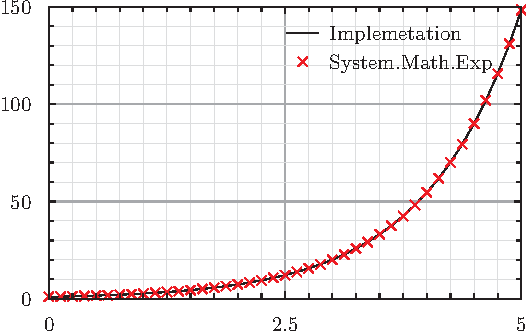
\includegraphics[width=\linewidth]{explot.pdf}
\end{figure}

\section{Itroduction}

The exponential function is given by $f(x)=\text{exp}(x)$ or $e^{x}$ (where the argument x is written as an exponent). It's can be defined in multiple ways. Its commonly used in mathematics some might say that the exponential function is "the most important function in mathematics". 

\section*{Implementation}

In this short report we will investigate, the Taylor-series for the exponential function \eqref{eq:taylor}.  

\begin{equation} \label{eq:taylor}
	e^x-1=x+\frac {x^2}2 + \frac{x^3}6+\cdots +\frac{x^n}{n!}+\cdots.	
\end{equation}

The Taylor series of any function is an infinite series formulation of the function itself, and are commonly used to approximate functions. However, computing an infinite series would require an infinite amount of computations which poses quite a problem. In order to prevent this, the approximation used here only takes the first 10th terms. If a negative argument is passed to the function, eg. -x, it is run as $(e^{-x})^{-1}$. If the input argument is of greater precision than 1/8, the function is called recursively as $(e^{\frac{x}{2}})^2$ to maintain the desired precision. This should work since the taylor power series is a good approximation for small $x$ and we evaluate at 1/8, this and the fact that we increase the precision by calculating smaller exponentials and then scalling improves the appoximation further.

\section*{Results}

In order to test whether the 10th term Taylor series approximation \eqref{eq:taylor} works, it is compared to the C\# implemented function, System.Math.Exp. A comparison is illustrated in figure \ref{fig:ex}. Which shows that \eqref{eq:taylor} is a sufficient approximation.



\end{document}